\chapter{Qualitätssicherung}
\label{chap:Qualitätssicherung}
Die Qualität des Source-To-Source Compilers muss während und nach der erfolgreichen Implementierung sichergestellt werden. In diesem Kapitel werden im ersten Abschnitt die Komponententests als Qualitätsischerungsmaßnahme wärend der Entwicklung thematisiert.  Anschließend wird die Funktionsweise mithilfe einer speziell entwickelten Xamarin.Forms App überprüft.  Anhand dieses Maßnahmen kann anschließend überprüft werden, ob  der Compiler erwartungsgemäß arbeitet. 

\section{Komponententests}
Komponententests unterteilen ein Programm in einzelne,  testfähige Einheiten und validieren deren Funktionalität.  Wenn sie integraler Bestandteil des Entwicklungspozesses sind,  optimieren sie die Qualität des Programms.  In Visual Studio können diese Testfälle, bei Änderungen am Quelltext automatisiert durchgeführt 
werden, was garantiert, dass die Modifikation am Code kein unerwünschtes Verhalten erzeugt.   Sobald eine Klasse oder Methode geschrieben ist, beginnt die Analyse, die das Verhalten des Codes nach Eingabe von gültigen, falschen und grenzwertig gültigen Daten überprüft. 
Diese testgesteuerte (engl. testdriven) Entwicklung entspricht der Qualitätssicherung bei 
der Programmierung des Source-To-Source Compilers, denn auch hier wurden die Komponententests vor dem Quelltext geschrieben und dienen damit auch der funktionalen Spezifikation der Anforderungen.\footcite[Vgl.][Abgerufen am \today]{MicrosoftColor} 

Dieses Vorgehen wird an dieser Stelle anhand der Umwandlung von Farben exemplarisch dargelegt.  Durch verschiedene verfügbare Eingabeformate ist es notwendig,  dass der Compiler eine vollständige Umwandlung vornimmt.  App-Entwickler können die Farbe mit einem gültigen Farbnahmen oder als Hexadezimale Zahl angeben.  Die Hexadezimale Darstellung kann jeweils über drei, vier,  sechs oder acht Ziffern mit einem optionalen Präfix \# angegeben werden. \footcite[Vgl.][Abgerufen am \today]{MicrosoftColor} 
Anhand dieser Anforderungen können nun die in Quelltext \ref{lst:colorTest} gezeigten Testfälle entworfen worden.

\lstinputlisting[label={lst:colorTest},caption={Testfälle für die Umwandlung von Farben}, language=csh]{SourceCode/Testcases.cs}

Durch diese Testfälle unterstützt konnte nun der in Quelltext \ref{lst:colorTestAlgo} dargestellte Algorithmus realisiert werden,  bei dem alle Testfälle korrekt ausgeführt werden.
\newpage
\lstinputlisting[label={lst:colorTestAlgo},caption={Algorithmus für die Umwandlung von Farben}, language=csh]{SourceCode/AlgorithmusColor.cs}



\section{Testobjekt}
Die Testapp wurde mit der Version 5.0.0.2012 des Xamarin.Forms Frameworks realisiert und verwendet die Erweiterungen Xamarin. Essentials.  Als Testobjekt soll diese mobile Anwendung möglichst viele Funktionalitäten von Xamarin.Forms abbilden,  hat jedoch nicht den Anspruch einer vollständigen Testabdeckung.
Auf plattformspezifische Implementationen mit Ausnahme der Metadaten und Ressourcen wurde verzichtet.  Eine genaue Beschreibung der App-Funktionalitäten und -Eigenschaften folgt und wird mithilfe von iOS Screenshots veranschaulicht.  Die entsprechenden Android Screenshots befinden sich in \hyperref[chap:AnhangAndroidScreenshots]{Anhang III}.  Abbildung \ref{fig:TestObjectI} zeigt im ersten Screenshoot den Startbildschirm mit dem Namen und Icon der Testapp und im zweiten den Hauptbildschirm.  


\begin{figure}[!ht]
 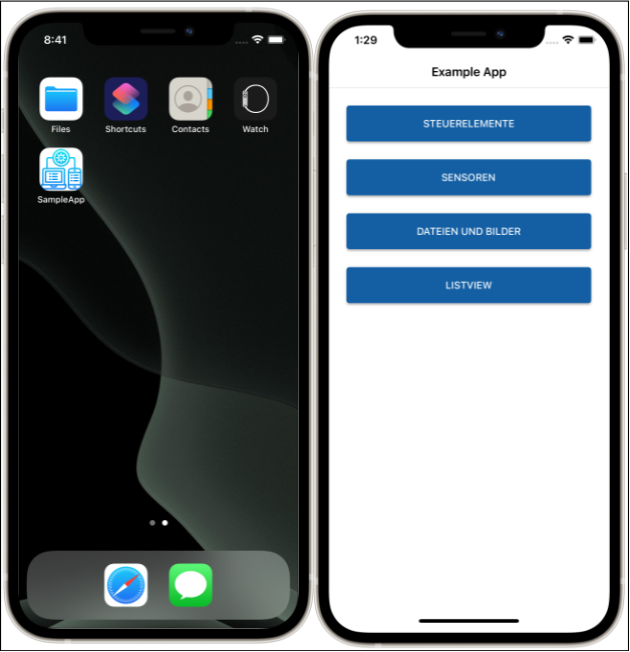
\includegraphics[width=\textwidth,keepaspectratio]{Images/Screenshot/AppIconAndMenu.png}
 \caption{Test Objekt Screenshots I}
 \label{fig:TestObjectI}
\end{figure}

Anhand des Namens,  SampleApp,  und eines Anwendungsicons können Anwender die App auf dem Startbildschirm identifizieren.  Nach ihrem Start öffnet sich eine Menüstruktur,  die Wurzel der Navigation, über die verschiedene Bereiche, der mobilen Anwendung angesteuert werden können.  In einer vertikal Ansicht werden dafür Schaltflächen als Ereignisauslöser für die Navigation bereitgestellt,  die zu den Seiten, Übersicht der Steuerelemente,  Ausgabe von Smartphonesensoren,  Arbeit mit Bildern und Ansicht einer Listview führt.   Abbildung \ref{fig:TestObjectII} zeigt die Übersicht der Steuerelemente sowie die Werte der Smartphone-Sensoren.

\begin{figure}[!ht]
 \includegraphics[width=\textwidth,keepaspectratio]{Images/Screenshot/Sensors.png}
 \caption{Test Objekt Screenshots II}
 \label{fig:TestObjectII}
\end{figure}
Die Übersicht zeigt einige der gängigsten Steuerelemente, die anhand der in Kapitel 4 aufgeführten 
Kategorien gruppiert und vertikal angeordnet wurden.  Zu den angezeigten Steuerelementen gehören neben einer Schaltfläche,  und einem Bild auch Auswahlmöglichkeiten für Datum und Uhrzeitwerte.  Neben dieser Darstellung ist im zweiten Screenshot eine Übersicht bezüglich der aktuellen Werte des Beschleunigungssensors und des Gyroskopes abgebildet,  die über das Plugin Xamarin.Essentials in der Codebehind-Datei ausgelesen werden. Anschließend werden die jeweiligen X, Y und Z-Achsenwerte über Databindings im \ac{ui} angezeigt.  Die nächsten beiden Screenshots in \ref{fig:TestObjectIII} zeigen das Menü für die Arbeit mit Bildern und einem zusätzlichen Berechtigungsdialog rechts.

\newpage 
\begin{figure}[!ht]
 \includegraphics[width=\textwidth,keepaspectratio]{Images/Screenshot/Permissions.png}
 \caption{Test Objekt Screenshots III}
 \label{fig:TestObjectIII}
\end{figure}
Das Menü hat Ähnlichkeiten mit dem der Hauptseite,  statt einer Navigation werden hier jedoch plattformspezifische Funktionalitäten über das Xamarin.Essentials Plugin ausgeführt die einen Zugriff auf die Kamera und die Galerie des Smartphones bieten.  Der Dialog,  der nach der Zugriffsberechtigung fragt zeigt auf iOS einen Eintrag aus den Metadaten an.
Die nächste Abbildung zeigt links im Screenshot die Auswahlfunktion von Bildern aus der Galerie,  vor welcher ebenfalls eine Berechtigung abgefragt wird, 
und rechts eine ListView mit Namen und E-Mail-Adressen von fiktiven Benutzern.  Die Klasse Benutzer wird innerhalb des Quelltexters der mobilen Anwendung definiert und über den Namespace in die Codebehind-Datei referenziert.  Anschließend werden exemplarisch zehn Objekte dieser Klasse innerhalb der Codebehind Datei in einer Auflistung vorgehalten und mithilfe eines Databindings in der ListView angezeigt. 
\newpage 
\begin{figure}[!ht]
 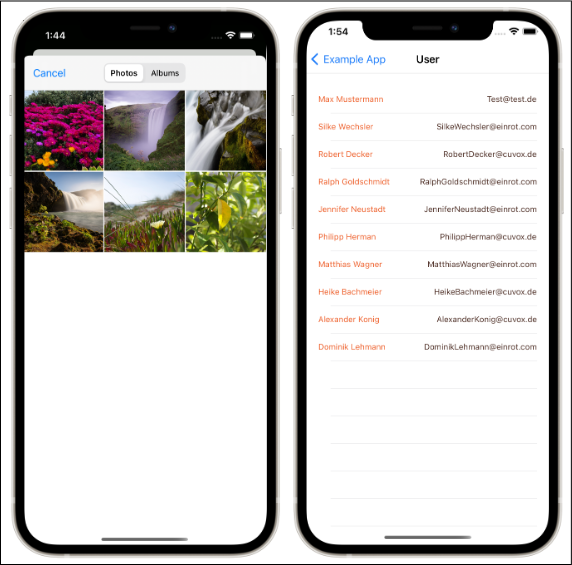
\includegraphics[width=\textwidth,keepaspectratio]{Images/Screenshot/ImagesListView.png}
 \caption{Test Objekt Screenshots IV}
 \label{fig:TestObjectIV}
\end{figure}


\section{Testfälle}
Zur Überprüfung der Funktionalität des Compilers müssen Testfälle definiert werden. Damit ist zu 
kontrollieren, ob die Übersetzung der in \Csharp{} programmierten  Xamarin.Forms Testapp eine in 
visuell und logisch vergleichbare Flutter Zielapp ergibt.  Diese manuell zu testenden Fälle leiten sich anhand der Funktionalitäten des Testobjektes ab.  Tabelle \ref{tab:Testapp} beschreibt die Testfälle und ihre entsprechenden Funktionen.

\newpage
\begin{xltabular}{\textwidth}{|l|X|}
\hline
   \textbf{Prüfobjekt} & \textbf{Prüfvorgang}  \\  
\hline
App-Icon	           					& Prüfen ob das App-Icon übernommen wurde                      			 		\\ 
App-Name          					& Prüfen ob das App-Name übernommen wurde                      		 \\ 
Seitenname  	         				& In der Navigationsleiste wird der Name der aktuellen Seite angezeigt               \\ 
Menü         			  				& Alle 4 Menüpunkte werden angezeigt                     			 \\ 
Navigation         			  		& Mit Hilfe des Menüs kann navigiert werden                      			 \\ 
Navigation          					& Über die Navigationsleiste kann zurück zur Navigationswurzel navigiert werden                      			 \\ 
Schriftgrößen			         	& Die Schriftgrößen in der Anwendungen wurden korrekt übernommen                 			 \\ 
Farben						         	& Die Farben in der Anwendung wurden korrekt übernommen                 			 \\ 
Layouts 								& Alle Layouts werden durch die entsprechenden Widgets ersetzt.                 			 \\ 
Steuerelemente						& Alle Steuerelemente werden durch die entsprechenden Widgets ersetzt.                 			 \\ 
Beschleunigungssensor        	& Die Werte des Beschleunigungssensor werden ausgegeben          			 \\ 
Gy­ro­s­kop						         & Die Werte des Gyroskopes werden ausgegeben                            			 \\ 
Kamera			         				& Es können Bilder mit der Kamera aufgenommen werden                			 \\ 
Galerie			         				& Es können Bilder aus der Kamera ausgewählt werden                			 \\ 
Berechtigungen			         	& Die Anwendung fragt nach der Berechtigung bei dem Zugriff auf Kamera und Galerie                   			 \\ 
ListView					         	& Die Listview wird mit den entsprechenden Daten angezeigt                   			 \\ 
\hline

	  \caption{Testfälle der Testapp}

 \label{tab:Testapp}
\end{xltabular}


\section{Testablauf}
Die Analyse der Softwarequalität erfolgt nicht ausschließlich automatisiert.  In diesem Abschnitt werden die definierten Testfälle durchgeführt und ihr Ergebnis dokumentiert.
Der Start  des Testlaufs beginnt mit dem Aufruf der grafischen Benutzeroberfläche,   der Auswahl der Xamarin.Forms Testapp und eines leeren Ordners, der als Zielverzeichnis nach der Kompilierung dient. 
Aufgrund der vielen Dateizugriffe und durchzuführenden Aktionen nimmt die Übersetzung der Anwendung eine gewisse Zeit in Anspruch. Im Frontend lassen sich Informationen über den Status, den Verlauf und mögliche Fehlerquellen nach der Übersetzung ablesen.  Anschließend kann die fertige Flutter Anwendung mithilfe der SDK kompiliert und ihre Ansichten kontrolliert werden.  Die im folgenden visualisierten Screenshots zeigen die generierte iOS Flutter-App,  die entsprechenden Androidrepräsenationen befinden Anhang dieser Arbeit.  Zur Förderung der Vergleichbarkeit werden die gleichen Inhalte der mobilen Anwendung abgebildet.  In Abbildung \ref{fig:FlutterAppI} wird links der Startbildschirm mit dem Namen und Icon und rechts das zentrale Menü der App dargestellt. 

\begin{figure}[!ht]
 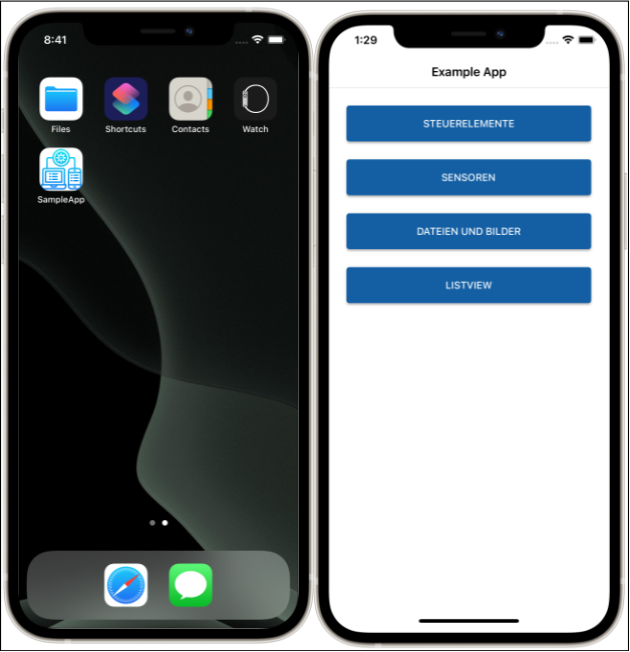
\includegraphics[width=\textwidth,keepaspectratio]{Images/Screenshot/AppIconAndMenu.png}
 \caption{Flutter App Screenshots I}
 \label{fig:FlutterAppI}
\end{figure}

Die Screenshots zeigen,  auf den ersten Blick die erwartete visuelle Vergleichbarkeit der Anwendungen.  Sowohl der Name als auch das Launchericon der Anwendung sind korrekt übernommen worden.  Nach dem Start der Anwendung fallen jedoch Designabweichungen auf, die durch die Verwendung der Material Design Vorlagen in Flutter begründet sind. Da der Compiler nicht,  wie in den Ausschlusskriterien festgelegt, den Style der Anwendung übersetzt,  entspricht das Ergebnis der Erwartungshaltung und ist, wenn daraus keine funktionellen Störungen 
entstehen,  an dieser Stelle akzeptabel.  Das zentrale Menü mit seiner Navigationsfunktion entspricht in der Ziel- dem der Testapp,  
unterscheidet sich, wenn auch nicht in der Abbildung ersichtlich,  in der Animation.  Abbildung \ref{fig:FlutterAppII} zeigt die Übersicht der Steuerelemente sowie die Werte der Smartphone-Sensoren.

\begin{figure}[!ht]
 \includegraphics[width=\textwidth,keepaspectratio]{Images/Screenshot/Sensors.png}
 \caption{Flutter App Screenshots II}
 \label{fig:FlutterAppII}
\end{figure}
Die übersetzten Übersicht der Steuerelemente stimmt  bezüglich der Verschachtlungen als auch der Funktionalitäten mit denen der Xamarin.Forms Variante überein,  was beispielsweise beim Öffnen der Datum- und Uhrzeitenauswahl erkennbar ist. Ebenfalls korrekt übernommen wurde die Oberfläche der Sensorenansicht und alle Werte der Smartphonesensoren befinden sich im richtigen Format. Im Gegensatz zu Xamarin.Forms werden diese Daten jedoch nicht im gleichen Zyklus aktualisiert.  Dieser Unterschied basiert auf den Implementationen des jeweiligen Plugins und entsteht nicht durch den Übersetzer.  In der Xamarin.Forms App würden die Werte über Databindings geladen und mithilfe der INotifyPropertyChanged Schnittstelle wurde die Benutzeroberfläche im Falle von Änderungen aktualisiert.  Die Schnittstelle wurde in der Flutter Anwendung entfernt und die Stellen des Quelltextes, die Änderungen am UI vornehmen mit einem Setstate-Block umschlossen damit sich die Oberfläche aktualisiert.  Die in Abbildung \ref{fig:FlutterAppIII}   gezeigten Screenshots zeigen ein Menue zur Arbeit mit Bildern, wobei der rechte zusätzlich den Berechtigungdialog für die Kameraverwendung bietet. 


  
\begin{figure}[!ht]
 \includegraphics[width=\textwidth,keepaspectratio]{Images/Screenshot/Permissions.png}
 \caption{Flutter App Screenshots III}
 \label{fig:FlutterAppIII}
\end{figure}
Der Berechtigungsdialog des rechten Screenshot entspricht nach Kompilierung in Darstellung und 
Funktion dem der Xamarin.Forms Version.  Auch der Zugriff auf die Kamera und die Galerie wurde, allerdings mithilfe der Erweiterung image\_picker, erfolgreich übersetzt.

Dieses funktioniert wie in der ursprünglichen Version des Testobjekts.  Die letzten Screenshots darstellt in Abbildung \ref{fig:TestObjectIV} zeigen,  die Auswahl eines Bildes aus der Galerie und die Darstellung der Benutzerdaten in einer ListView.  Die korrekte Darstellung der ListView beweist, dass auch die Klassendefinition und ihr
Konstruktor korrekt übersetzt wurden, denn nur unter dieser Voraussetzung konnte die Liste mit den 
passenden Daten gefüllt werden.

 
  
\begin{figure}[!ht]
 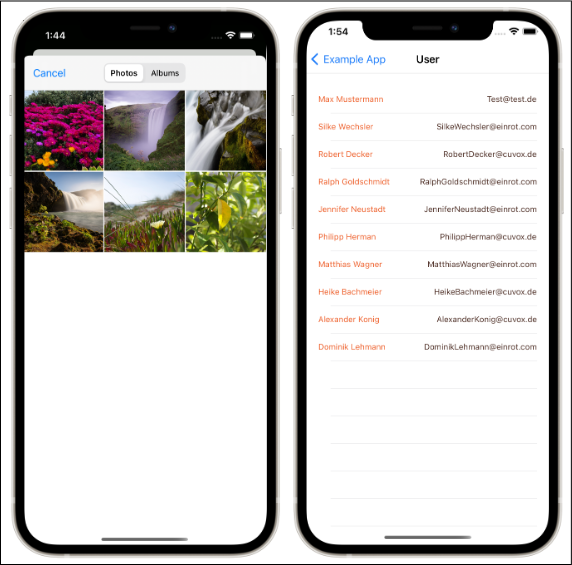
\includegraphics[width=\textwidth,keepaspectratio]{Images/Screenshot/ImagesListView.png}
 \caption{Flutter App Screenshots IV}
 \label{fig:FlutterAppIV}
\end{figure}

Das Testobjekt konnte vollständig überführt werden, was grundsätzlich die 
Funktionsfähigkeit die Prototypen beweist. Bei einer Übersetzung aller in der Praxis möglichen 
Funktionalitäten von Xamerin.Forms bedarf es vielfältiger Erweiterungen des Compilers.

 Auch wenn die Erstellungen von Webseiten nicht im Fokus dieser Arbeit steht, soll diese 
Anwendung Möglichkeit trotzdem kurz betrachtet werden, da sie seit März 2021 mit der 
 von Flutter 2.0. besteht und somit eine vergleichbare Darstellung auf 
großen Bildschirmen wie z.B. PCs und Laptops möglich ist. Da Xamarin.Forms Apps, also auch die Testapp nicht diese Darstellungsoption auf großen 
Monitoren adäquat abgebildet, wird die übersetzte Flutter App ebenfalls nicht optimal im Web präsentiert,  ist aber trotzdem 
lauffähig. Einschränkungen der Webfunktionalitäten resultieren nicht nur aus dem Übersetzungsvorgang, 
sondern sind dem erst seit einigen Wochen bestehenden Support der Webplattform und der noch 
nicht vollständigen Aktualisierung aller Erweiterungen geschuldet.  Es fehlt der Zugriff auf die Sensoren und das Plugin für die Verwendung der Kamera.   Abbildung \ref{fig:WebView} zeigt einen Screenshot der Webanwendung.
\begin{figure}[!ht]
 \includegraphics[width=\textwidth,keepaspectratio]{Images/Implementation/WebApp.png}
 \caption{Flutter Web-App Screenshot}
 \label{fig:WebView}
\end{figure}




